% Toolbar icon: remesh (MMG) — a coarse triangle turned into a finer
% triangulation of the same shape (uniform refinement), with an arrow between.
\documentclass[tikz,border=2mm]{standalone}
\usetikzlibrary{arrows.meta,calc,shapes.geometric}
\begin{document}
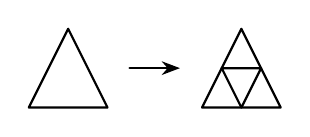
\begin{tikzpicture}[line width=1.3pt, line cap=round, line join=round, >=Stealth, x=1mm,y=1mm]
  % --- coarse triangle ---
  \coordinate (A) at (-16,-5);
  \coordinate (B) at (-6,-5);
  \coordinate (C) at (-11,5);
  \draw[thick] (A) -- (B) -- (C) -- cycle;
  % --- arrow ---
  \draw[thick,->] (-3.2,0) -- (3.2,0);
  % --- refined triangle (subdivided into 4) ---
  \coordinate (D) at (6,-5);
  \coordinate (E) at (16,-5);
  \coordinate (F) at (11,5);
  \coordinate (DE) at ($(D)!0.5!(E)$);
  \coordinate (EF) at ($(E)!0.5!(F)$);
  \coordinate (FD) at ($(F)!0.5!(D)$);
  \draw[thick] (D) -- (E) -- (F) -- cycle;
  \draw[thick] (DE) -- (EF) -- (FD) -- cycle;
\end{tikzpicture}
\end{document}
